\section{Performance Experiment}
\subsection{Overview}
Huffman Encoding optimizes storage by assigning shorter bit representations to more frequently occurring characters in the provided text data. While Huffman Encoding can be applied to any binary file, this test focuses specifically on ASCII text for simplicity. The test data is generated using predefined character sets to analyze how different character distributions impact compression efficiency. The code used to generate these test files is provided for reproducibility.
\subsection{Testing procedure}
\begin{itemize}
    \item \textbf{Test File Generation}: generate the test file using a predefined character set.
    \item \textbf{Huffman Encoding and Decoding}: the generated test file is encoded using Huffman Encoding algorithm and then decoded back to its original form.
    \item \textbf{Verification}: compare the input file and the decoded version to ensure the correctness of the implemented Huffman Encoding algorithm.
    \item \textbf{Data Collection}: saving the size of the input file, encoded version for further analysis.
\end{itemize}
\subsection{Dataset Description}
\begin{itemize}
    \item The dataset consists of four different input sizes: 500, 2000, 100000, and 10000000 characters.
    \item The generated text files are based on four predefined character sets: \begin{itemize}
        \item "\textbf{Lower}": Only lowercase letters and whitespace (28 unique characters).
        \item "\textbf{LowerUpper}": Includes both lowercase and uppercase letters (54 unique characters).
        \item "\textbf{ASCII}": Contains lowercase, uppercase, digits and whitespace (64 unique characters).
        \item "\textbf{Printable}": Includes all printable ASCII characters (97 unique characters).
    \end{itemize}
\end{itemize}
\subsection{Result}
\begin{figure}[H]
    \centering
    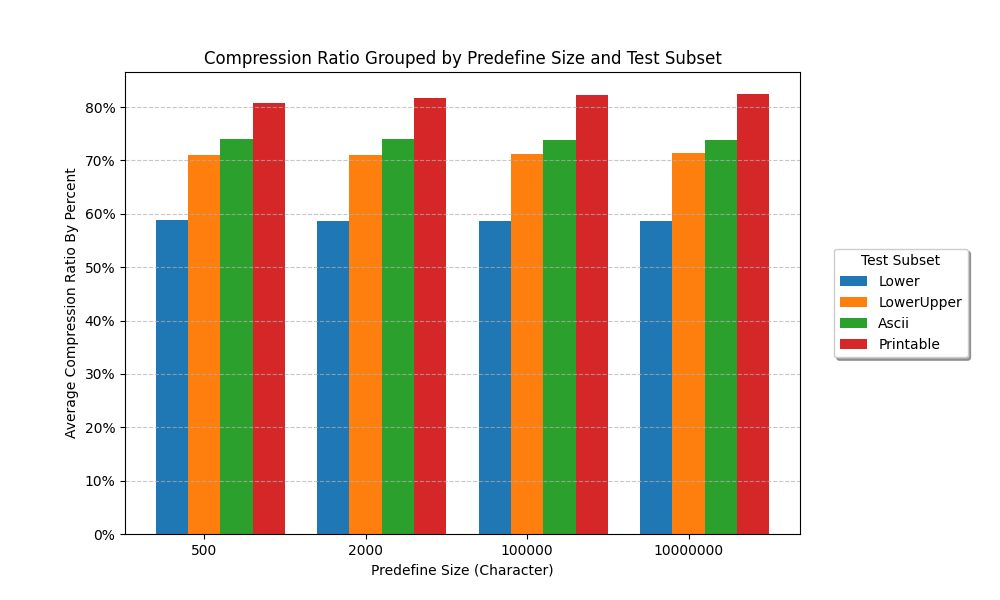
\includegraphics[width=1\linewidth]{total.png}
    \caption{Compression Ratio Group by File size and Character set}
    \label{fig:Compression-Ratio}
\end{figure}
\begin{itemize}
    \item This graph is presented as part of the experimental evaluation of a Huffman coding implementation. It visually summarizes the compression performance achieved across different input file sizes and character sets. The y-axis represents the "\textbf{Average Compression Ratio By Percent}" which we'll define precisely below. The x-axis groups the results by "\textbf{Predefined Size by Character}" representing the total number of characters in the input files. Within each size group, there are four bars, each representing a different "\textbf{Test Subset}" (character set).
    \item The compression ratio is calculated using the formula: 
\[Compression Ratio = (Encoded File Size / Original File Size) * 100\%\]
\textbf{A lower compression ratio is better}, indicating a greater reduction in file size. A ratio of 100\% means that there are no compression; a ratio of 50\% indicate that the encoded file is half the size of the original. A ratio above 100\% would imply that the "\textbf{compressed}" file is actually larger than the original (which is possible with Huffman coding if the input data has a very uniform distribution of characters).
    \item The graph shows four distinct file size groups: 500, 2000, 100000 and 10000000 characters. Within each character set, the compression ratio remains consistent across these different file sizes. This suggests the effectiveness of Huffman Coding is largely \textbf{independent of overall file size}. 
    \item \textbf{The strong dependence of the compression ratio on the character set is directly due to the structure of the Huffman tree}. Larger character sets, particularly those with many low-frequency characters, result in taller trees and longer average code lengths, decreasing the compression efficiency.
\end{itemize}
\subsection{Conclusion}
These results confirm that Huffman Coding is an effective lossless compression technique for ASCII text files. Under standard conditions (Printable character set), Huffman Encoding reduces file size by approximately 20\%. In specific cases, such as datasets with highly repetitive characters, the reduction can be as high as 30\%.